% multiple1902 <multiple1902@gmail.com>
% intro.tex
% Copyright 2011~2012, multiple1902 (Weisi Dai)
% https://code.google.com/p/xjtuthesis/
% 
% It is strongly recommended that you read documentations located at
%   http://code.google.com/p/xjtuthesis/wiki/Landing?tm=6
% in advance of your compilation if you have not read them before.
%
% This work may be distributed and/or modified under the
% conditions of the LaTeX Project Public License, either version 1.3
% of this license or (at your option) any later version.
% The latest version of this license is in
%   http://www.latex-project.org/lppl.txt
% and version 1.3 or later is part of all distributions of LaTeX
% version 2005/12/01 or later.
%
% This work has the LPPL maintenance status `maintained'.
% 
% The Current Maintainer of this work is Weisi Dai.
%
%\chapter{绪论}
%\echapter{Preface}
\chapter{Preface}

\section{Physicochemical Properties}
Lysozyme (EC 3.2.1.17) is a protein existing in animals, plants, bacteria, and viruses. It can be found in neutrophils, macrophage granules, serum, saliva, milk, honey, and eggs. The enzyme hydrolyzed β-1,4 glycosidic bond between N-acetyl muramic acid (NAM) and N-acetyl glucosamine (NAG) of cytoderm peptidoglycan (PG) in Gram-positive and Gram-negative bacteria \citep{Gajda2014}. C-type lysozyme of egg white is a model for studying protein structure and function. 

\subsection{Structure and Mechanism}

The three-dimensional structure of lysozyme was first resolved in 1965 by X-ray \citep{Blake1965}. Lysozyme consists of 129 amino acids cross-linked by 4 disulfide bonds, and lysozyme has two main domains. The α domain of the molecule is mainly composed of α helix, while the β domain contains β fold and helix. The active site is in the gap between the two domains. 

There are two catalytic mechanisms to explain lysozyme. According to the Phillips mechanism, two residues Glu35 (glutamic acid) and Asp52 (aspartic acid) play an important role. The terminal proton of Glu35 is transferred to the O atom of the glycosidic bond between two adjacent sugar residues, which leads to cleavage of glycosidic bond and formation of a carbocation. The positive charge of the carbocation is stabilized by the negative charge of Asp52 until the hydroxide ion binds to the positive C atom and Glu35 is protonated. Another is Intermediate theory. Like all other retained β-glucosidases, egg white lysozyme proceeds through the formation of covalent intermediates and subsequent decomposition rather than through the formation of long-lived ion pairs \citep{Vocadlo2001}. The latest research supports the Phillips mechanism more \citep{Held2014}.

\begin{figure}[!h]
	\centering
	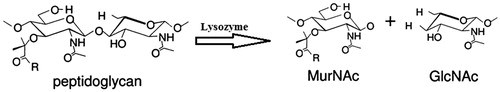
\includegraphics[width=0.9\linewidth]{figures/chp1_lysozyme_mechanism}
	\caption{The Reaction. Extracted from \cite{Ercan2016}}
	\label{fig:chp1lysozymemechanism}
\end{figure}

\subsection{Function and Applications}
Lysozyme has broad-spectrum resistance to both Gram-negative and Gram-positive bacteria. The bactericidal ability of lysozyme is not only due to its catalytic activity but also due to its cationic and hydrophobic characteristics \citep{Pellegrini1992}. Chemical modifications such as oleoyl chloride \citep{Evran2010} and Na2SO3 \citep{Liu2018} can enhance the hydrophobic properties of lysozyme and enhance its antibacterial effect. Research \citep{Ibrahim2001} proved that the helix-loop-helix domain located in the 87–114 sequence of lysozyme and its C-terminal helix domain passed through the outer membrane and damaged the inner membrane through self-promoting absorption, thus killing Gram-negative bacteria. In the human body, lysozyme degrades bacteria not only by directly killing bacteria but also by releasing immune regulatory bacterial ligands including PG fragments to participate in the regulation of the immune system \citep{ragland2017bacterial}. PG fragment can eliminate bacteria by enhancing the activation of phagocytes.

Egg white is composed of lysozyme, accounting for about 0.5\% of its weight. At present, egg white lysozyme occupies a dominant position in the market, and its main limitations are high recovery cost, low activity, and immunological problems \citep{Ercan2016}. This immunological problem is dominated by IgE \citep{Urisu2015}, and people who are allergic to eggs will cause immunological problems, so the production of human lysozyme is also an important research direction. At present, the human lysozyme gene is expressed in heterologous organisms, such as rice \citep{R.Wilken2011} and yeast \citep{Huang2009}. Studies in rice have proved that the manufacturing cost (\$/g) is the same as that of eggs \citep{R.Wilken2011}.



\section{Discussion on the Application}
Given the ability to lyse the cell wall of bacterial,
lysozyme has been attracting immense attention as a kind of 
environment-friendly or organs-friendly antimicrobial.
As we have discussed before, it has nowadays more and more applications in the food industry and clinical procedures. In this part, we will discuss 
it's applications within our preparations and capabilities.

\subsection{Applications in Food Industry}
Our first focus is on the food industry. Since the 1800s when Napoléon launched his strategy to conquer Europe, the storage or preservation of food has become a major question in the food industry. Sealing food in cans, High-temperature treatment, Pasteurization, numerous methods had risen. And in the last, people introduced chemical additives to the food industry. Efficient as it is, nowadays people are having less tolerance in that chemical industry. Due to the conception of eating healthy, they prefer so-called "Non-additive food" to chemical treated food. But the lack of bacterial inhibition will easily make it a perfect bacterial petri dish. The chemical hazard vanishes, but the microbial hazard just arises. We need another method!

So we cast our sight to the biological method to preserve food. In our case, we are planning to introduce lysozyme to food packing and food additives. As for the food packing, we are going to distribute the lysozyme agent, in gluten \citep{Conte2006} or onto a chitosan powder, on the food packages, mostly LDPE, these methods have been taken into practice \citep{Borzooeian2017}. And its function to extend to the shelf life of foods had been proved \citep{Lian2012, Alhazmi2014}. our points of view, this kind of application suits our capability very well, and we have put it into our first consideration.

Another important application in the food industry is the food additive. We can add some lysozyme into specific easy-deteriorating foods, such as wurst, can-foods, and diary. The addition of lysozyme will significantly extend the preserve half-life of food, these lysozymes are presented into chitosan particals \citep{Wu2017}, this will not only protect the original flavour of the food but also enhance its ability to inhibit bacterial emerging.

\subsection{Clinical Applications}
The lysozyme can also play an impressive role in the clinical procedure. Like the food industry, medical is also a battel against bacterial. In 1676, Anton van Leeuwenhoek observed bacteria and other microorganisms, using a single-lens microscope of his design.
In 1796, Edward Jenner developed a method using cowpox to successfully immunize a child against smallpox. The same principles are used for developing vaccines today.
Following on from this, in 1857 Louis Pasteur also designed vaccines against several diseases such as anthrax, fowl cholera and rabies as well as pasteurization for food preservation.
In 1867 Joseph Lister is considered to be the father of antiseptic surgery. By sterilizing the instruments with diluted carbolic acid and using it to clean wounds, post-operative infections were reduced, making surgery safer for patients.
In 1929 Alexander Fleming developed the most commonly used antibiotic substance both at the time and now: penicillin \citep{Brock2003}.The emerge of antibiotic medicine start a new era for human, we can sometimes beat the infection of microbes.

But there still exists a fatal problem: ALLERGY. Some antibiotics will lead to an acute allergic phenomenon, which is sometimes fatal. So we come up with this idea to introduce lysozyme to health-care products. We want to introduce it in for instance dentifrices, mouth-rinses, moisturizing gels, chewing gums or such sterilization products \citep{Tenovuo2002}.
We try to develop a kind of lysozyme covered bandage in which the lysozyme exist in gel, or in other advanced status, such as carbon nanotubes.

These are our prospects of the clinical application of lysozyme.


%应用的原理也说一点。让老师感觉有用(但也就是个大概。老师看了能提意见?

%\section{溶菌酶的应用}
\section{Applications of Lyzoenzymes}
%溶菌酶在食品、医药、生物技术等方面都有广泛的应用
Here we conducted a summary of current research on the application of lysozymes. We find that our two ideas are practical and potentially valuable in our daily life. Today lysozymes have been widely applied to food, medical, and biological industries. 

%\subsection{食品和发酵}
\subsection{Applications in Food and Fermentation Industry}

%我国食品工业生产过程中广泛使用化学合成防腐剂,它们对人体可能有潜在的毒副作用;而溶菌酶就是一种天然防腐剂。
%溶菌酶本身对人体没有毒害作用,缺可以很好地抑制细菌的生长,有效地延长食品的保质期。
Natural lysozymes can repress bacterial growth without undermining our health thus they are mainly used as preservatives. \citet{ZHAI2015} demonstrate in their review that lysozymes can prevent cheese from microorganism-caused swelling during the production; they also have an outstanding effect in retaining the freshness of meat product combined with other natural preservatives.
\citet{Yu-tong2006} and \citet{ZHAI2015} all show that lysozymes are added into Japanese sake (a kind of low wine) to replace salicylic acid or \ce{SO2} in as the preservative. Microorganisms are initiators of aquatic products' rotting. \citet{Ren2013} point out in their review that lysozymes may do better than instant cool storage with the help of some other techniques like ultrahigh pressure.

%\citet{ZHAI2015}在其综述中发现,“溶菌酶和其他天然防腐剂复合而成的保鲜剂,在鲜肉和熟制肉品的保鲜过程中确实有明显的效果”;干酪生产过程中,微生物的发酵会导致干酪的膨胀,而添加溶菌酶能抑制这种微生物的生长。微生物也是引起水产品腐败变质的主要原因,\citet{Ren2013}在其综述中指出,溶菌酶的应用使得某些水产品的保存效果优于冷藏,但需要配合多种溶菌酶或其他保存措施使用

\subsection{Applications in Medical Industry}
Lysozymes are a component of the second line of immune defense in our body for their nonspecific bactericidal effect. Moreover, people are adding extra lysozymes to strengthen our immune system or cure inflammation and infection. Lysozymes can also improve the therapeutic effect of various kinds of drugs. 

According to \cite{Yu-tong2006} and \cite{ZHAI2015}, lysozymes can regulate gut microbes by specifically killing putrefactive ones and selectively increase the number of bifidobacterium, which is a significant intestinal probiotic. Therefore, lysozymes bring remission to enteritis and enhance the immune system. It is pretty helpful for susceptible infants.  Adding lysozyme to milk is widely applied as a quality-improvement strategy.
Lyzozymes extracted from egg white are also made into industralized mouth wash, which can inhibit the growth of over 99\% \textit{Escherichia coli} and \textit{Staphylococcus aureus} \citep{Unknown2020}.
%但溶菌酶也不是要杀灭所有微生物,相反,还具有调节肠道微生物的功能。它对肠道中腐败性微生物有特殊的杀灭作用,却促进双歧杆菌的生长。双歧杆菌是一种重要的肠道有益微生物,为人体提供生物屏障和营养、免疫增强作用。在乳制品中加入溶菌酶,可以平衡肠道菌群、缓解肠炎,对婴幼儿有着尤其突出的效果。所以,往往可向溶菌酶含量较低的牛乳中添加溶菌酶,同时起到抑菌的作用。
%从蛋清提取的溶菌酶制成的漱口水有巨大的市场潜力,该漱口水对大肠杆菌和金黄色葡萄球菌的抑制率达99\%以上\citep{Unknown2020}。

%\citet{He2008}综述了溶菌酶在医药中的应用,主要包括:抑制口腔龋齿的生长,对表层性溃疡、对真菌感染、烧伤创面感染、疱疹的治疗效果好于传统抗真菌药物,还有治疗SARS病毒感染、作为肿瘤治疗助剂的潜力。
\citet{He2008} also reviewed applications in the medical industry, listed as follows:
\begin{itemize}
	\item Inhibition of dental caries growth;
	\item Treatment of surface ulcers, fungal infection, burn wound infection, and herpes (with a better than traditional antifungal drugs);
	\item Treatment of SARS virus infection;
	\item Potential as a tumor treatment adjuvant.
\end{itemize}

%\subsection{其他领域}
\subsection{Other Applications}
%将溶菌酶与高分子物质结合有着巨大的应用价值和开发前景。\cite{Le-chuan2020}综述了溶菌酶与高分子等形成的复合材料的应用。溶菌酶和多糖、蛋白、多酚等的结合,能提高其抗菌活性,增强其使用稳定性,拓宽其应用范围。现在它们已经用于制造抗菌包装材料(食品)、可控释膜材料、特殊纳米材料(用于医药)等。 
Attaching lysozymes to polymers is of great application value and worth deeper study. \cite{Le-chuan2020} reviewed applications of those composites. Polymers like polysaccharide, protein, and polyphenol, etc. enhance the bactericidal activity, stability, and range of application of lysozymes. With their excellent biocompatibility, \citet{Lin2015} constructed a lysozyme/pectin complex for drug delivery with satisfying results.
%构建了一种溶菌酶/果胶纳米凝胶并用于抗癌药物递送,取得了较好的效果。

Lysozymes also play an important role in gene engineering as a kind of tool enzyme. They remove the cell wall of Gram-positive bacteria, and protoplast is obtained for cell fusion or cellular matter extraction \citep{Yu-tong2006}.

%\subsection{应用的局限性}
\subsection{Limitations}
Although lysozymes are extensively studied, there remain problems to be solved. As a natural product, separation and purification methods still needs perfection. Industrialized production is still under development and the cost is still high \citet{ZHAI2015}. \citet{Zhao2009} state in their review that natural lysozymes don't have a wide antibacterial spectrum. Some propose that protein-modification might be useful, but the biosafety cannot be guaranteed and protein structure should be studied. At the same time, cooperation, optimal adding proportion, and working condition between lysozymes and other preservatives are still under further research \citep{ZHAI2015}.

%溶菌酶虽已被广泛研究,却也还存在一些问题没能很好地解决。这种天然产物的分离提纯、工业化生产还不成熟,成本也较高\citet{ZHAI2015}。\citet{Zhao2009}在其综述中指出,天然溶菌酶的抑菌谱不够广,尤其是革兰氏阴性菌,一些学者提出用蛋白质修饰的手段来扩展之;但他们也认为,修饰后的溶菌酶的安全性有待商榷,蛋白质结构有待深入研究。同时,溶菌酶与其他食品防腐剂的协同作用、配比优化、最适条件等还有待研究\citet{ZHAI2015}。

